\section{Iniciando e parando Pbinds independentemente}

Está é uma dúvida muito comum que surge com \texttt{Pbind}s, especialmente as que rodam para sempre com \texttt{inf}: como posso parar e iniciar \texttt{Pbind}s quando eu quiser? A resposta envolverá o uso de variáveis e veremos um exemplo completo em breve, mas antes de chegarmos lá, precisamos entender um pouco melhor o que acontece quando você toca um \texttt{Pbind}.

\subsection{Pbind como uma partitura musical}

Você pode pensar no \texttt{Pbind} como uma espécie de partitura musical: é uma receita para fazer sons, um conjunto de instruções para realizar uma passagem musical. Para que a partitura se torne música, você precisa entregá-la a um intérprete: alguém que vai ler a partitura e fazer sons com base nessas instruções. Vamos separar conceitualmente estes dois momentos: a definição da partitura e a performance da mesma.
 
\begin{lstlisting}[style=SuperCollider-IDE, basicstyle=\scttfamily\footnotesize]
// Defina a partitura
(
p = Pbind(
	\midinote, Pseq([57, 62, 64, 65, 67, 69], inf),
	\dur, 1/7
); // sem .play aqui!
)

// Peça que a partitura seja tocada
p.play;
\end{lstlisting}
 

A variável \texttt{p} no exemplo acima simplesmente guarda a partitura---perceba que o \texttt{Pbind} não tem uma mensagem \texttt{.play} logo após o fechamento dos parênteses. Nenhum som é feito neste ponto. O segundo momento é quando você pede ao SuperCollider que toque a partitura: \texttt{p.play}.

Um erro comum neste ponto é tentar \texttt{p.stop}, na esperança de parar o tocador. Tente isso e verifique por si mesmo que não funciona deste jeito. Você entenderá o porquê nos próximos parágrafos.

\subsection{EventStreamPlayer}

Limpe a Post window com [ctrl+shift+P] (não é absolutamente necessário, mas por que não?) e rode \texttt{p.play} novamente. Olhe para a Post window e você verá que o resultado é algo chamado  \texttt{EventStreamPlayer} (“Tocador de fluxo de eventos”). Toda vez que você chama um \texttt{.play} em um \texttt{Pbind}, o SuperCollider cria um tocador que realiza aquela ação: o \texttt{EventStreamPlayer} é isso. É como ter um pianista se materializando na sua frente toda vez que você disser “Eu quero que esta partitura seja tocada agora”. Legal, né?


Bem, sim, exceto pelo fato de que depois que este tocador virtual anônimo aparece e começa seu trabalho, você não tem mais como falar com ele---ele não tem nome. Em termos ligeiramente mais técnicos, você criou um objeto, mas você não tem como se referir a este objeto depois. Talvez neste ponto você pode ver porque \texttt{p.stop} não funciona: é como tentar falar com a partitura em vez de falar com o tocador. A partitura (o \texttt{Pbind} armazenado na variável \texttt{p}) não sabe nada sobre começar ou parar: ela é só uma receita. O \emph{tocador} é quem sabe sobre tocar, parar, “por favor volte do começo”, etc. Em outras palavras, você tem que falar com o \texttt{EventStreamPlayer}. Tudo que você precisa fazer é dar um nome a ele, ou seja, armanzená-lo em uma variável:

 
\begin{lstlisting}[style=SuperCollider-IDE, basicstyle=\scttfamily\footnotesize]
// Experimente estas linhas, uma por uma:
~meuTocador = p.play;
~meuTocador.stop;
~meuTocador.resume;
~meuTocador.stop.reset;
~meuTocador.start;
~meuTocador.stop;
\end{lstlisting}
 

Em resumo: chamando \texttt{.play} em um \texttt{Pbind} gera um \texttt{EventStreamPlayer}; e armazenando seu \texttt{EventStreamPlayer}s em variáveis permite que você os acesse mais tarde para iniciar e parar Patterns individualmente (sem precisar usar [ctrl+.], que interrompe tudo de uma vez).

\subsection{Exemplo}

Aqui temos um exemplo mais complexo para finalizar esta seção. A melodia superior é emprestada do “Álbum para a Juventude” de Tchaikovsky e uma melodia mais grave é adicionada em contraponto. A figura \ref{fig:counterpoint} mostra a passagem em notação musical.
 
%\lstinputlisting[style=SuperCollider-IDE, basicstyle=\scttfamily\footnotesize]{code-pbind-start-stop.scd}

\begin{lstlisting}[style=SuperCollider-IDE, basicstyle=\scttfamily\footnotesize]
// Defina a partitura
(
var minhasDurs = Pseq([Pn(1, 5), 3, Pn(1, 5), 3, Pn(1, 6), 1/2, 1/2, 1, 1, 3, 1, 3], inf) * 0.4;
~melodiaSuperior = Pbind(
	\midinote, Pseq([69, 74, 76, 77, 79, 81, Pseq([81, 79, 81, 82, 79, 81], 2), 82, 81, 79, 77, 76, 74, 74], inf),
	\dur, minhasDurs
);
~melodiaInferior = Pbind(
	\midinote, Pseq([57, 62, 61, 60, 59, 58, 57, 55, 53, 52, 50, 49, 50, 52, 50, 55, 53, 52, 53, 55, 57, 58, 61, 62, 62], inf),
	\dur, minhasDurs
);
)
// Toque as duas juntas:
(
~tocador1 = ~melodiaSuperior.play;
~tocador2 = ~melodiaInferior.play;
)
// Pare-os separadamente:
~tocador1.stop;
~tocador2.stop;
// Outras mensagens disponíveis
~tocador1.resume; // retomar
~tocador1.reset; //voltar do início
~tocador1.play;
~tocador1.start; // mesmo que .play
\end{lstlisting}

\begin{figure}[h]
\centerline{\framebox{
	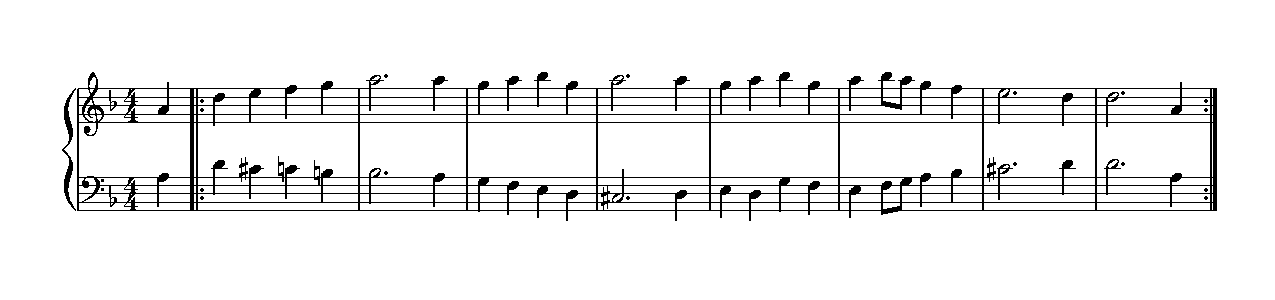
\includegraphics[scale=0.7]{code-pbind-start-stop-notation.pdf}}}
\caption{\texttt{Pbind} contraponto com uma melodia de Tchaikovsky}
\label{fig:counterpoint}
\end{figure}

Primeiro, perceba o uso de variáveis. Uma delas, \texttt{minhasDurs}, é uma variável local. Você pode dizer que é uma variável local porque não começa com um til ($\sim$) e é declarada no início com a palavra-chave específica \texttt{\textbf{var}}. Esta variável guarda toda um \texttt{Pseq} que será usada como \texttt{\textbackslash dur} em ambos os \texttt{Pbind}s. \texttt{minhasDurs} é necessária somente no momento de definir a partitura, então faz sentido usar uma variável local para isso (embora uma variável global funcionasse igualmente bem). As outras variáveis que você vê no exemplo são variáveis globais---uma vez declaradas, são válidas em qualquer lugar nos seus patches de SuperCollider.

Segundo, perceba a separação ente partitura e tocadores, como discutimos anteriormente. Quando os \texttt{Pbind}s são definidos, eles não são tocados no mesmo momento---não há \texttt{.play} imediatamente depois de fechar os parênteses. Depois que você roda o primeiro bloco de código, tudo o que você tem são duas definições de \texttt{Pbind} armazenadas nas variáveis \texttt{$\sim$melodiaSuperior} e \texttt{$\sim$melodiaInferior}. Elas ainda não fazem som---são apenas partituras. A linha \texttt{$\sim$tocador1 = $\sim$melodiaSuperior.play} cria um \texttt{EventStreamPlayer} para cumprir a tarefa de tocar a melodia superior e a este tocador é dado o nome $\sim$tocador1. A mesma ideia vale para o $\sim$tocador2. Graças a isso, podemos falar com cada tocador e pedi-lo para parar, iniciar, retomar, etc.

Com o risco de soar tedioso, vamos reiterar uma última vez:
\begin{itemize}
\item Um \texttt{Pbind} é só uma receita para fazer som, como uma partitura musical;
\item Quando você chama a mensagem \texttt{play} em um \texttt{Pbind}, um objeto \texttt{EventStreamPlayer} é criado;
\item Se você armazena este \texttt{EventStreamPlayer} em uma variável, você pode acessá-lo mais tarde para usar comandos como \texttt{stop} e \texttt{resume}.
\end{itemize} 
